\documentclass[border=2pt]{standalone}
\usepackage{tikz}
\usetikzlibrary{datavisualization.formats.functions}
\begin{document}
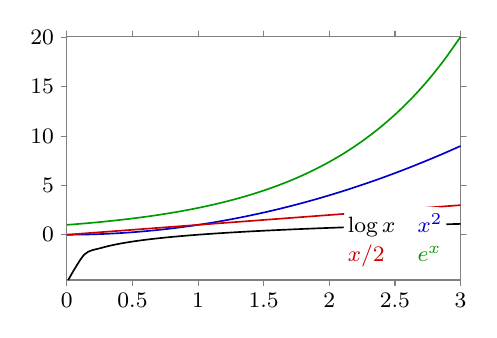
\begin{tikzpicture}
\datavisualization data group {function classes} = {
  data [format=function,set=log] {
    var x : interval [0.01:3];
    func y = ln(\value x);
  }
  data [format=function,set=lin] {
    var x : interval [0:3];
    func y = \value x;
  }
  data [format=function,set=squared] {
    var x : interval [0:3];
    func y = \value x * \value x;
  }
  data [format=function,set=exp] {
    var x : interval [0:3];
    func y = exp(\value x);
  }
};
\datavisualization [
  scientific axes,
  visualize as smooth line/.list={log,lin,squared,exp},
  legend={south east inside,rows=2,label style=text only},
  log={label in legend={text=$\log x$}},
  lin={label in legend={text=$x/2$}},
  squared={label in legend={text=$x^2$}},
  exp={label in legend={text=$e^x$}},
  style sheet=strong colors]
data group {function classes};
\end{tikzpicture}
\end{document}
